\chapter{Plannung und Dürchführung} \label{plannung_durchfuhrung}
% [X] Chapter Einführung
Dieser Kapitel ist in zwei Unterkapiteln aufgeteilt, der Entwicklungsprozess und der Entwurf. Im ersteren wird darauf eingegangen, wie die Entwicklung des Projektes abgelaufen ist, mit Emphase auf Anforderungen, Betriebsmodi, funktionelle Architektur und die Softwarestruktur. Im zweiteren werden Designaspekten jeder Anforderung beleuchtet, wobei diese technisch beschrieben und mit Auszügen des Quellcodes kontextualisiert werden.  

\section{Entwicklungsprozess} \label{Entwicklungsprozess}

\subsection{Anforderungsdefinition}
\begin{figure}[H]\centering
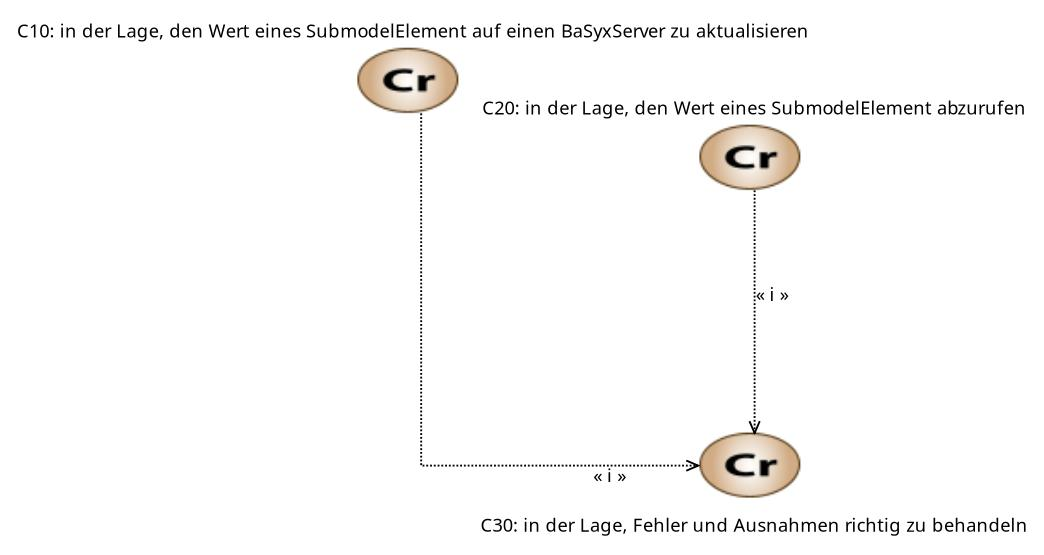
\includegraphics[width=10cm,height=10cm,keepaspectratio]{media/diagrams/CRB.jpg}
\caption{Capabilities Diagram)}
\label{fig:CRB}
\end{figure}

\subsection{Funktionale Spezifikation}

\section{Entwurf} \label{Entwurf}

% Beschreibung jedes Capabilities des Projektes
% - Problemstellung und Motivation
% - Methodologie
% - Endarchitektur
\subsection{Wrappen des BaSyx als S-Function}

